% Uebung Leistungsberechnung  nach Brinkmeyer
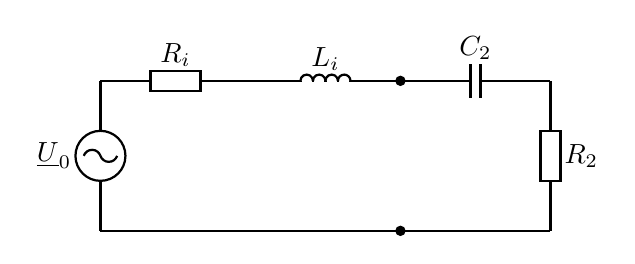
\begin{tikzpicture}[scale=2.54]%
% dpic version 2024.01.01 option -g for TikZ and PGF 1.01
\ifx\dpiclw\undefined\newdimen\dpiclw\fi
\global\def\dpicdraw{\draw[line width=\dpiclw]}
\global\def\dpicstop{;}
\dpiclw=0.8bp
\dpiclw=0.8bp
\dpicdraw (0,0)
 --(0.25,0)\dpicstop
\dpicdraw (0.5,0)
 --(0.5,0.05)
 --(0.25,0.05)
 --(0.25,-0.05)
 --(0.5,-0.05)
 --(0.5,0)\dpicstop
\dpicdraw (0.5,0)
 --(0.75,0)\dpicstop
\draw (0.375,0.05) node[above=-2bp]{$ R_i$};
\dpicdraw (0.75,0)
 --(1,0)\dpicstop
\dpicdraw (1,0)
 --(1,-0.005556)\dpicstop
\dpicdraw (1,-0)
 ..controls (1,0.011165) and (1.005956,0.021481)
 ..(1.015625,0.027063)
 ..controls (1.025294,0.032646) and (1.037206,0.032646)
 ..(1.046875,0.027063)
 ..controls (1.056544,0.021481) and (1.0625,0.011165)
 ..(1.0625,0)\dpicstop
\dpicdraw (1.0625,0)
 --(1.0625,-0.005556)\dpicstop
\dpicdraw (1.0625,-0)
 ..controls (1.0625,0.011165) and (1.068456,0.021481)
 ..(1.078125,0.027063)
 ..controls (1.087794,0.032646) and (1.099706,0.032646)
 ..(1.109375,0.027063)
 ..controls (1.119044,0.021481) and (1.125,0.011165)
 ..(1.125,0)\dpicstop
\dpicdraw (1.125,0)
 --(1.125,-0.005556)\dpicstop
\dpicdraw (1.125,-0)
 ..controls (1.125,0.011165) and (1.130956,0.021481)
 ..(1.140625,0.027063)
 ..controls (1.150294,0.032646) and (1.162206,0.032646)
 ..(1.171875,0.027063)
 ..controls (1.181544,0.021481) and (1.1875,0.011165)
 ..(1.1875,0)\dpicstop
\dpicdraw (1.1875,0)
 --(1.1875,-0.005556)\dpicstop
\dpicdraw (1.1875,0)
 ..controls (1.1875,0.017259) and (1.201491,0.03125)
 ..(1.21875,0.03125)
 ..controls (1.236009,0.03125) and (1.25,0.017259)
 ..(1.25,0)\dpicstop
\dpicdraw (1.25,0)
 --(1.25,-0.005556)\dpicstop
\dpicdraw (1.25,0)
 --(1.5,0)\dpicstop
\draw (1.125,0.03125) node[above=-2bp]{$ L_i$};
\dpicdraw[fill=black](1.5,0) circle (0.007874in)\dpicstop
\dpicdraw[fill=black](1.5,-0.75) circle (0.007874in)\dpicstop
\dpicdraw (1.5,0)
 --(1.85,0)\dpicstop
\dpicdraw (1.85,-0.083333)
 --(1.85,0.083333)\dpicstop
\dpicdraw (1.9,-0.083333)
 --(1.9,0.083333)\dpicstop
\dpicdraw (1.9,0)
 --(2.25,0)\dpicstop
\draw (1.875,0.083333) node[above=-2bp]{$ C_2$};
\dpicdraw (2.25,0)
 --(2.25,-0.25)\dpicstop
\dpicdraw (2.25,-0.5)
 --(2.3,-0.5)
 --(2.3,-0.25)
 --(2.2,-0.25)
 --(2.2,-0.5)
 --(2.25,-0.5)\dpicstop
\dpicdraw (2.25,-0.5)
 --(2.25,-0.75)\dpicstop
\draw (2.3,-0.375) node[right=-2bp]{$ R_2$};
\dpicdraw (0,0)
 --(0,-0.25)\dpicstop
\dpicdraw (0,-0.375) circle (0.049213in)\dpicstop
\dpicdraw (-0,-0.375)
 ..controls (-0.005978,-0.357065) and (-0.022762,-0.344968)
 ..(-0.041667,-0.344968)
 ..controls (-0.060571,-0.344968) and (-0.077355,-0.357065)
 ..(-0.083333,-0.375)\dpicstop
\dpicdraw (0,-0.375)
 ..controls (0.005978,-0.392935) and (0.022762,-0.405032)
 ..(0.041667,-0.405032)
 ..controls (0.060571,-0.405032) and (0.077355,-0.392935)
 ..(0.083333,-0.375)\dpicstop
\dpicdraw (0,-0.5)
 --(0,-0.75)\dpicstop
\draw (-0.125,-0.375) node[left=-2bp]{$ \underline{U}_0$};
\dpicdraw (0,-0.75)
 --(2.25,-0.75)\dpicstop
\end{tikzpicture}%
